\documentclass{report}
\usepackage[utf8]{inputenc}

%----- Configuración del estilo del documento------%
\usepackage{epsfig,graphicx}
\usepackage[left=2.5cm,right=2.5cm,top=1.8cm,bottom=2.3cm]{geometry}
%------ Paquetes matematicos --------%
\usepackage{amsmath}
\usepackage{amssymb}
\usepackage{amsthm}
\usepackage{amsmath}
\usepackage{tabularx}
\usepackage{fancyhdr}
\usepackage{lastpage}
\usepackage{verbatim}
\usepackage[shortlabels]{enumitem}
\usepackage{venndiagram}
\usetikzlibrary{shapes.geometric}
\usepackage{cancel}
\usepackage{hyperref}
\usepackage[T1]{fontenc}
\usepackage[spanish,es-nodecimaldot,es-tabla]{babel}
\usepackage{csquotes}
\usepackage{graphicx}
\usepackage{tocloft}
\graphicspath{{./figs/}}
\usepackage{setspace}

% paquetes para bibliografia
\usepackage[backend=biber]{biblatex}
\addbibresource{resources/referencias/referencias.bib}

% paquetes para codigo 
\usepackage{listings}
\usepackage{xcolor}
\definecolor{keywords}{RGB}{0,0,180}
\definecolor{comments}{RGB}{0,128,0}
\definecolor{strings}{RGB}{163,21,21}

\lstdefinelanguage{SQL}{
    keywords={SELECT, FROM, WHERE, JOIN, ON, AS, ORDER,BY,OR, COUNT, CASE, WHEN, GROUP, END, DESC, THEN},
    keywordstyle=\color{keywords}\bfseries,
    commentstyle=\color{comments},
    stringstyle=\color{strings},
    morecomment=[l][\color{comments}]{--,/*,*/},
    morestring=[b]',
    sensitive=false
}

\lstset{
    language=SQL,
    basicstyle=\ttfamily,
    keywordstyle=\color{keywords}\bfseries,
    commentstyle=\color{comments},
    stringstyle=\color{strings},
    numbers=left,
    numberstyle=\tiny\color{gray},
    stepnumber=1,
    numbersep=10pt,
    showspaces=false,
    showstringspaces=false,
    tabsize=4,
    breaklines=true,
    frame=lines
}


\begin{document}
	
    % Portada del documento
	\begin{titlepage}
	\thispagestyle{empty}
	\begin{minipage}[c][0.17\textheight][c]{0.25\textwidth}
		\begin{center}
			
\includegraphics[width=3.5cm, height=3.5cm]{resources/Logo_UNAM.png}
		\end{center}
	\end{minipage}
	\begin{minipage}[c][0.195\textheight][t]{0.75\textwidth}
		\begin{center}
			\vspace{0.3cm}
			\textsc{\large Universidad Nacional Aut\'onoma de M\'exico}\\[0.5cm]
			\vspace{0.3cm}
			\hrule height2.5pt
			\vspace{.2cm}
			\hrule height1pt
			\vspace{.8cm}
			\textsc{Facultad de Ciencias}\\[0.5cm] %
		\end{center}
	\end{minipage}
	
	\begin{minipage}[c][0.81\textheight][t]{0.25\textwidth}
		\vspace*{5mm}
		\begin{center}
			\hskip2.0mm
			\vrule width1pt height13cm 
			\vspace{5mm}
			\hskip2pt
			\vrule width2.5pt height13cm
			\hskip2mm
			\vrule width1pt height13cm \\
			\vspace{5mm}
			
\includegraphics[height=4.0cm]{resources/Logo_FC.png}
		\end{center}
	\end{minipage}
	\begin{minipage}[c][0.81\textheight][t]{0.75\textwidth}
		\begin{center}
			\vspace{1cm}
			
			{\large\scshape Fundamentos de Bases de Datos - 7094}\\[.2in]
			
			\vspace{2cm}            
			
			\textsc{\LARGE \textbf{T}\hspace{1cm}\textbf{A}\hspace{1cm}\textbf{R}\hspace{1cm}\textbf{E}\hspace{1cm}\textbf{A}\hspace{1cm}\hspace{1cm}\textbf{4}}\\[2cm]
			\textsc{\Large{Equipo:}\normalsize \\
                \vspace{.3cm}
				\textbf{Del Monte Ortega Maryam Michelle - 320083527 \\
                \vspace{.2cm}
				\href{https://github.com/JuanSosaCiencias}{\textcolor{blue}{Sosa Romo Juan Mario - 320051926}} \\
                \vspace{.2cm}
				Castillo Hernández Antonio - 320017438 \\
                \vspace{.2cm}
                Erik Eduardo Gómez López - 320258211 \\
                \vspace{.2cm}
                Julio César Islas Espino - 320340594}}\\[0.5cm]     
			
			\textsc{{Fecha de entrega: \\ \textbf{10 de Octubre de 2024}}}\\[0.5cm]        
			
			\textsc{{Profesor: \\ \textbf{M. en I. Gerardo Avilés Rosas}}}\\[0.5cm]  
			
			\textsc{Ayudantes: \\ \textbf{Luis Enrique García Gómez \\ Kevin Jair Torres Valencia \\ Ricardo Badillo Macías \\ Rocío Aylin Huerta González
			} }
			
			
			\vspace{0.5cm}
		\end{center}
	\end{minipage}
\end{titlepage}


    % Titulo
	\begin{center}
		\section*{\LARGE{Práctica 9 : Consultas SQL}}
	\end{center}

    % Consultas
    \begin{section}{Consultas}
    \begin{enumerate}
        \item \textbf{Entrenadores y Atletas, que compartan el apellido y que se encuentren participando en la misma disciplina.
Deberan ordenar la información a partir del apellido paterno.}\vspace{.3cm}
        \item \section*{Consulta 2: Cantidad de asistentes y ganancias por disciplina y localidad}

\subsection*{Descripción}
Esta consulta calcula cuántas personas asistieron y cuánto dinero se ganó en cada disciplina y localidad. Es útil para evaluar el éxito financiero y la popularidad de los eventos en distintas áreas.

\textbf{SQL}

\begin{verbatim}
SELECT 
    d.NombreDisciplina,
    l.NombreLocalidad,
    SUM(e.Precio) AS GananciasTotales,
    COUNT(ce.IDCliente) AS CantidadAsistentes
FROM 
    Evento e
JOIN 
    Disciplina d ON e.IDDisciplina = d.IDDisciplina
JOIN 
    Localidad l ON e.NombreLocalidad = l.NombreLocalidad AND e.IDDisciplina = l.IDDisciplina
JOIN 
    CompraEntrada ce ON e.IDEvento = ce.IDEvento
GROUP BY 
    d.NombreDisciplina, l.NombreLocalidad
ORDER BY 
    CantidadAsistentes DESC;
\end{verbatim}

\begin{center}
    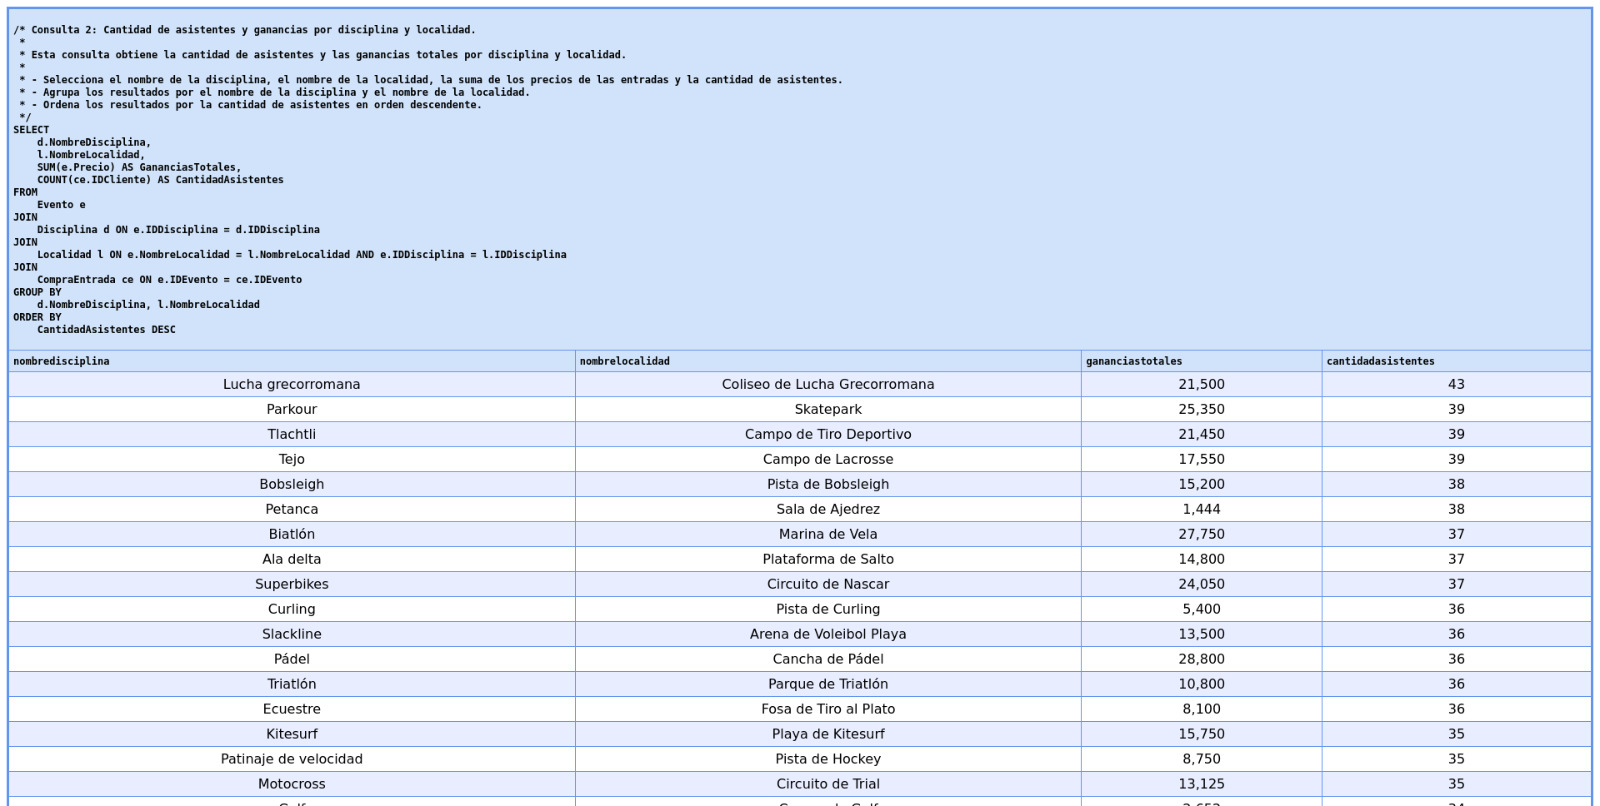
\includegraphics[width=16.5cm]{../resources/Chapters/Consultas/Imagenes/Consulta2.jpeg} 
    
   Consulta 2. Cantidad de asistentes y ganancias por disciplina y localidad. 
\end{center}

\textbf{Desglose de la consulta}

\begin{itemize}
   \item \textbf{Selección de columnas (\texttt{SELECT})}:
   \begin{itemize}
       \item Se seleccionan las siguientes columnas:
       \begin{itemize}
           \item \texttt{d.NombreDisciplina}: Nombre de la disciplina.
           \item \texttt{l.NombreLocalidad}: Nombre de la localidad.
           \item \texttt{SUM(e.Precio)}: Suma de los precios de las entradas, denominada \texttt{GananciasTotales}.
           \item \texttt{COUNT(ce.IDCliente)}: Cuenta la cantidad de asistentes, denominada \texttt{CantidadAsistentes}.
       \end{itemize}
   \end{itemize}
   
   \item \textbf{Tablas involucradas (\texttt{FROM} y \texttt{JOIN})}:
   \begin{itemize}
       \item La consulta utiliza cuatro tablas:
       \begin{itemize}
           \item \texttt{Evento (e)}: Contiene la información de los eventos.
           \item \texttt{Disciplina (d)}: Contiene la información de las disciplinas.
           \item \texttt{Localidad (l)}: Contiene la información de las localidades.
           \item \texttt{CompraEntrada (ce)}: Contiene la información de las entradas compradas.
       \end{itemize}
       \item Se realizan \texttt{JOINs} entre las tablas para relacionar los eventos con las disciplinas, localidades y entradas compradas.
   \end{itemize}
   
   \item \textbf{Agrupación de resultados (\texttt{GROUP BY})}:
   \begin{itemize}
       \item Para calcular la cantidad de asistentes y las ganancias por disciplina y localidad, se agrupan los datos según las columnas:
       \begin{itemize}
           \item \texttt{d.NombreDisciplina}, \texttt{l.NombreLocalidad}.
       \end{itemize}
       \item Esto garantiza que se genere un registro único por cada combinación de disciplina y localidad.
   \end{itemize}
   
   \item \textbf{Ordenamiento de resultados (\texttt{ORDER BY})}:
   \begin{itemize}
       \item Los resultados se ordenan por la columna \texttt{CantidadAsistentes} en orden descendente (\texttt{DESC}), de modo que las combinaciones de disciplina y localidad con más asistentes aparezcan primero.
   \end{itemize}
\end{itemize}

\textbf{Análisis detallado}

\begin{enumerate}
   \item \textbf{Relación entre tablas:}
   \begin{itemize}
       \item La consulta asume que existe una relación directa entre las tablas \texttt{Evento}, \texttt{Disciplina}, \texttt{Localidad} y \texttt{CompraEntrada} a través de las claves foráneas.
       \item Esto implica que:
       \begin{itemize}
           \item Cada evento está asociado con una disciplina y una localidad.
           \item Cada entrada comprada está asociada con un evento.
       \end{itemize}
   \end{itemize}
   
   \item \textbf{Uso de funciones agregadas \texttt{SUM} y \texttt{COUNT}:}
   \begin{itemize}
       \item La función \texttt{SUM(e.Precio)} calcula las ganancias totales generadas por las entradas vendidas para cada combinación de disciplina y localidad.
       \item La función \texttt{COUNT(ce.IDCliente)} cuenta el número de asistentes para cada combinación de disciplina y localidad.
   \end{itemize}
   
   \item \textbf{Agrupación por disciplina y localidad:}
   \begin{itemize}
       \item El uso de \texttt{GROUP BY} permite agrupar los registros por disciplina y localidad, asegurando que las ganancias y la cantidad de asistentes se calculen correctamente para cada combinación.
   \end{itemize}
   
   \item \textbf{Ordenamiento:}
   \begin{itemize}
       \item El orden descendente por \texttt{CantidadAsistentes} facilita la identificación de las combinaciones de disciplina y localidad con mayor número de asistentes.
   \end{itemize}
\end{enumerate}

\textbf{Consideraciones}

\begin{itemize}
   \item \textbf{Empates en la cantidad de asistentes:}
   \begin{itemize}
       \item Si varias combinaciones de disciplina y localidad tienen la misma cantidad de asistentes, el orden relativo entre ellas no está definido. Para resolver esto, se podría agregar un criterio adicional en el \texttt{ORDER BY}, como las ganancias totales.
   \end{itemize}
\end{itemize}

        \item \textbf{Atletas que hayan participado en más de 1 disciplina.}\vspace{.3cm}
        \item 
Cómo modificarías el diagrama de la figura a) para representar las siguientes restricciones:\\
Un alumno no puede tomar clase en más de una materia con el mismo profesor. Una materia no puede ser
impartida por más de un profesor.

No es necesario realizar alguna modificación, pues la cardinalidad uno a uno que tiene el diagrama implica que un alumno no puede estar relacionado con el mismo profesor en más de una materia, y del mismo modo una materia no puede ser impartida por más de un profesor en la relación, por lo que el diagrama ya cumple con ambas restricciones.

        \item \begin{center}
    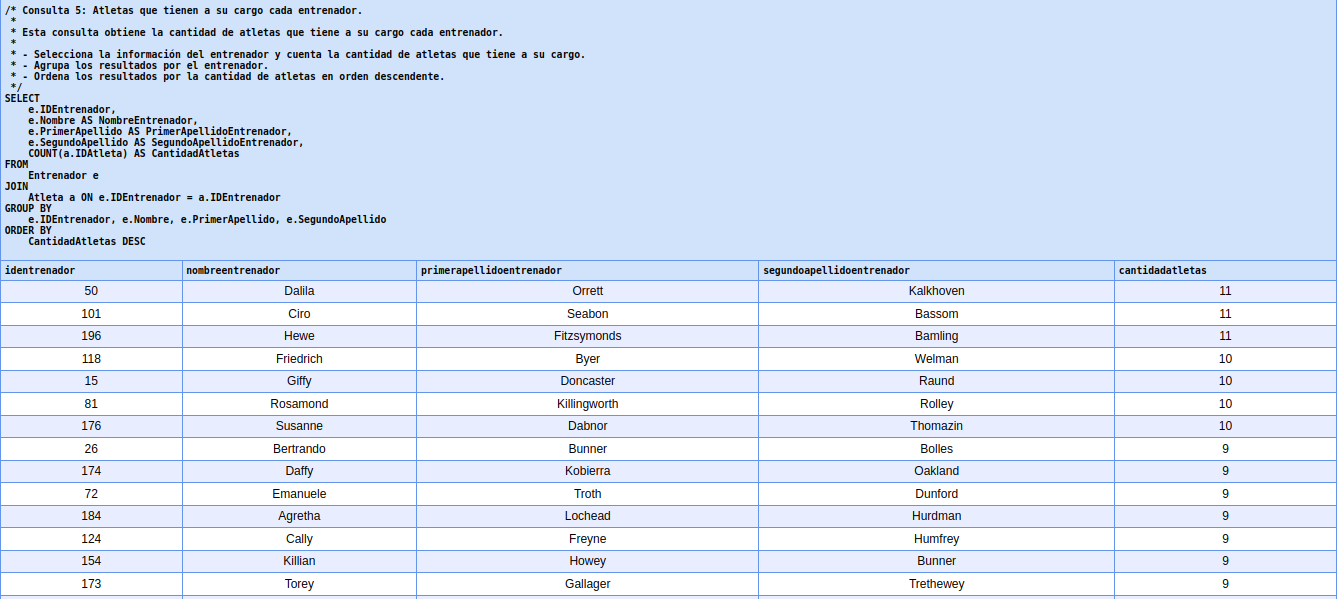
\includegraphics[width=16.5cm]{../resources/Chapters/Consultas/Imagenes/Consulta5.png} 
    
   Consulta 5. Atletas que tienen a su cargo cada entrenador. 
\end{center}

\textbf{Propósito de la consulta}

La consulta tiene como objetivo obtener un listado de entrenadores junto con la cantidad de atletas que tienen a su cargo. Esto es útil para entender la distribución de atletas entre los entrenadores y detectar posibles desequilibrios en la asignación de recursos.

\textbf{Desglose de la consulta}

\begin{itemize}
   \item \textbf{Selección de columnas (\texttt{SELECT})}:
   \begin{itemize}
       \item Se seleccionan las siguientes columnas del entrenador:
       \begin{itemize}
           \item \texttt{e.IDEntrenador}: Identificador único del entrenador.
           \item \texttt{e.Nombre}: Nombre del entrenador.
           \item \texttt{e.PrimerApellido}: Primer apellido del entrenador.
           \item \texttt{e.SegundoApellido}: Segundo apellido del entrenador.
       \end{itemize}
       \item Se utiliza la función agregada \texttt{COUNT(a.IDAtleta)} para contar cuántos atletas están asociados con cada entrenador. Esta columna se denomina \texttt{CantidadAtletas}.
   \end{itemize}
   
   \item \textbf{Tablas involucradas (\texttt{FROM} y \texttt{JOIN})}:
   \begin{itemize}
       \item La consulta utiliza dos tablas:
       \begin{itemize}
           \item \texttt{Entrenador (e)}: Contiene la información de los entrenadores.
           \item \texttt{Atleta (a)}: Contiene la información de los atletas.
       \end{itemize}
       \item Se realiza un \texttt{JOIN} entre ambas tablas utilizando la relación \texttt{e.IDEntrenador = a.IDEntrenador}. Esto asegura que solo se consideren los atletas que están asignados a un entrenador.
   \end{itemize}
   
   \item \textbf{Agrupación de resultados (\texttt{GROUP BY})}:
   \begin{itemize}
       \item Para calcular la cantidad de atletas por entrenador, se agrupan los datos según las columnas únicas del entrenador:
       \begin{itemize}
           \item \texttt{e.IDEntrenador}, \texttt{e.Nombre}, \texttt{e.PrimerApellido}, \texttt{e.SegundoApellido}.
       \end{itemize}
       \item Esto garantiza que se genere un registro único por cada entrenador.
   \end{itemize}
   
   \item \textbf{Ordenamiento de resultados (\texttt{ORDER BY})}:
   \begin{itemize}
       \item Los resultados se ordenan por la columna \texttt{CantidadAtletas} en orden descendente (\texttt{DESC}), de modo que los entrenadores con más atletas aparezcan primero.
   \end{itemize}
\end{itemize}

\textbf{Análisis detallado}

\begin{enumerate}
   \item \textbf{Relación entre tablas:}
   \begin{itemize}
       \item La consulta asume que existe una relación directa entre las tablas \texttt{Entrenador} y \texttt{Atleta} a través de la clave foránea \texttt{a.IDEntrenador}, que apunta a \texttt{e.IDEntrenador}.
       \item Esto implica que:
       \begin{itemize}
           \item Cada atleta tiene asignado exactamente un entrenador.
           \item Un entrenador puede tener asignados uno o más atletas.
       \end{itemize}
   \end{itemize}
   
   \item \textbf{Uso de la función agregada \texttt{COUNT}:}
   \begin{itemize}
       \item La función \texttt{COUNT(a.IDAtleta)} cuenta el número de registros en la tabla \texttt{Atleta} que están relacionados con cada entrenador.
       \item Si un entrenador no tiene atletas asignados, no aparecerá en los resultados porque el \texttt{JOIN} elimina las filas sin coincidencias.
   \end{itemize}
   
   \item \textbf{Agrupación por entrenador:}
   \begin{itemize}
       \item El uso de \texttt{GROUP BY} permite agrupar los registros por entrenador, asegurando que la cantidad de atletas se calcule correctamente para cada uno.
   \end{itemize}
   
   \item \textbf{Ordenamiento:}
   \begin{itemize}
       \item El orden descendente por \texttt{CantidadAtletas} facilita la identificación de los entrenadores con mayor carga de trabajo.
   \end{itemize}
\end{enumerate}

\textbf{Consideraciones}

\begin{itemize}
   
   \item \textbf{Empates en la cantidad de atletas:}
   \begin{itemize}
       \item Si varios entrenadores tienen la misma cantidad de atletas, el orden relativo entre ellos no está definido. Para resolver esto, se podría agregar un criterio adicional en el \texttt{ORDER BY}, como el nombre del entrenador.
   \end{itemize}
\end{itemize}

        \item \begin{center}
    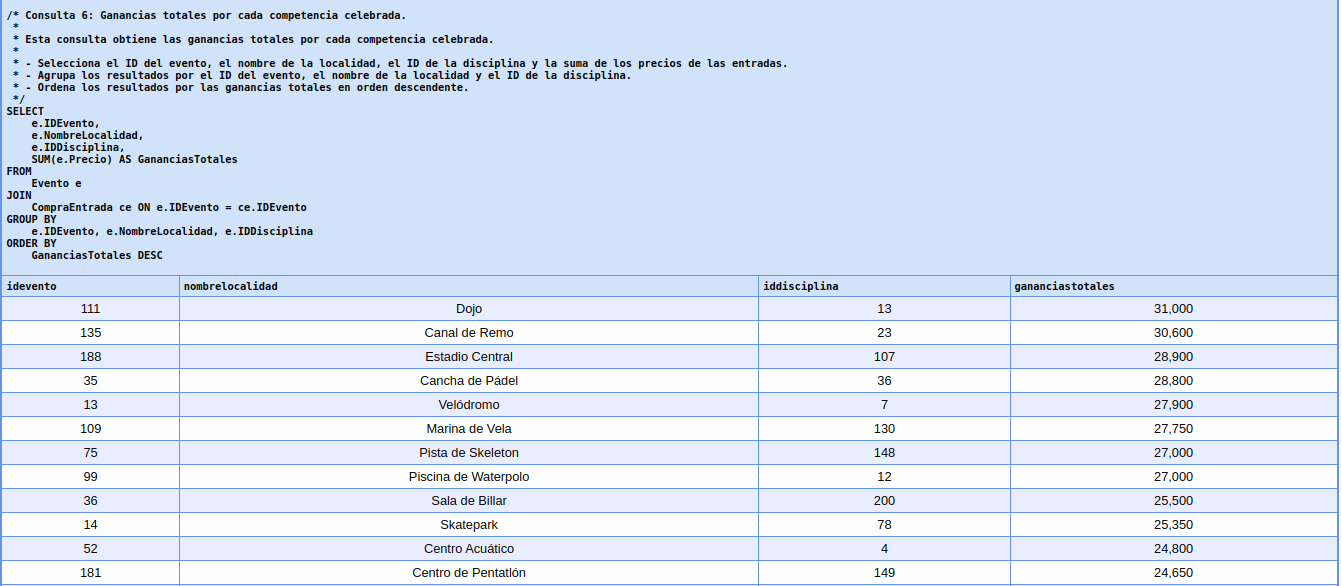
\includegraphics[width=16.5cm]{resources/Chapters/Consultas/Imagenes/Consulta6.png} 
    
   Consulta 6. Ganancias totales por cada competencia celebrada.
\end{center}

\textbf{Propósito de la consulta}

La consulta tiene como objetivo calcular las ganancias totales generadas por la venta de entradas para cada competencia celebrada. Esto permite identificar qué eventos fueron más rentables y en qué localidades o disciplinas se generaron mayores ingresos.

\textbf{Desglose de la consulta}

\begin{itemize}
   \item \textbf{Selección de columnas (\texttt{SELECT}):}
   \begin{itemize}
       \item \texttt{e.IDEvento}: Identificador único del evento, que permite distinguir cada competencia.
       \item \texttt{e.NombreLocalidad}: Nombre de la localidad donde se celebró el evento.
       \item \texttt{e.IDDisciplina}: Identificador de la disciplina deportiva asociada al evento.
       \item \texttt{SUM(e.Precio) AS GananciasTotales}: Calcula la suma total de los precios de las entradas vendidas para cada evento, representando las ganancias totales.
   \end{itemize}

   \item \textbf{Tablas involucradas (\texttt{FROM} y \texttt{JOIN}):}
   \begin{itemize}
       \item \texttt{Evento (e)}: Contiene información sobre los eventos celebrados, como su identificador, localidad y disciplina.
       \item \texttt{CompraEntrada (ce)}: Registra las compras de entradas realizadas para los eventos.
       \item \textbf{Unión (\texttt{JOIN})}: Se realiza un \texttt{JOIN} entre ambas tablas utilizando la relación \texttt{e.IDEvento = ce.IDEvento}, asegurando que solo se consideren las entradas compradas para eventos específicos.
   \end{itemize}

   \item \textbf{Agrupación de resultados (\texttt{GROUP BY}):}
   \begin{itemize}
       \item La agrupación se realiza por las siguientes columnas:
       \begin{itemize}
           \item \texttt{e.IDEvento}: Para agrupar las ganancias por cada evento específico.
           \item \texttt{e.NombreLocalidad}: Para asociar las ganancias con la localidad donde se celebró el evento.
           \item \texttt{e.IDDisciplina}: Para distinguir las ganancias según la disciplina deportiva del evento.
       \end{itemize}
       \item Esto permite calcular la suma de los precios de las entradas (\texttt{SUM(e.Precio)}) de manera independiente para cada combinación de evento, localidad y disciplina.
   \end{itemize}

   \item \textbf{Ordenamiento de resultados (\texttt{ORDER BY}):}
   \begin{itemize}
       \item Los resultados se ordenan por la columna \texttt{GananciasTotales} en orden descendente (\texttt{DESC}), de modo que los eventos con mayores ganancias aparezcan primero.
   \end{itemize}
\end{itemize}

\textbf{Análisis detallado}

\begin{itemize}
   \item \textbf{Relación entre tablas:}
   \begin{itemize}
       \item La consulta asume que existe una relación directa entre las tablas \texttt{Evento} y \texttt{CompraEntrada} mediante la clave foránea \texttt{ce.IDEvento}, que apunta a \texttt{e.IDEvento}.
       \item Esto implica que cada entrada comprada está asociada a un único evento y que un evento puede tener múltiples entradas compradas.
   \end{itemize}

   \item \textbf{Uso de la función agregada \texttt{SUM}:}
   \begin{itemize}
       \item La función \texttt{SUM(e.Precio)} calcula la suma total de los precios de las entradas vendidas para cada evento.
       \item Se supone que el campo \texttt{Precio} en la tabla \texttt{Evento} representa el precio de una entrada individual y que este valor se multiplica implícitamente por el número de entradas compradas en la tabla \texttt{CompraEntrada}.
   \end{itemize}

   \item \textbf{Agrupación por columnas clave:}
   \begin{itemize}
       \item La agrupación por \texttt{e.IDEvento}, \texttt{e.NombreLocalidad} y \texttt{e.IDDisciplina} asegura que las ganancias se calculen de manera específica para cada combinación de:
       \begin{itemize}
           \item Evento único (\texttt{e.IDEvento}).
           \item Localidad donde se celebró el evento (\texttt{e.NombreLocalidad}).
           \item Disciplina deportiva asociada al evento (\texttt{e.IDDisciplina}).
       \end{itemize}
   \end{itemize}

   \item \textbf{Ordenamiento por ganancias:}
   \begin{itemize}
       \item Ordenar los resultados por \texttt{GananciasTotales} en orden descendente permite identificar fácilmente los eventos más rentables.
   \end{itemize}
\end{itemize}

\textbf{Posibles escenarios y consideraciones}

\begin{itemize}
   \item \textbf{Eventos sin entradas vendidas:}
   \begin{itemize}
       \item Si un evento no tiene entradas vendidas, no aparecerá en los resultados debido al \texttt{JOIN}. Esto significa que solo se mostrarán eventos con al menos una entrada comprada.
   \end{itemize}

   \item \textbf{Localidades y disciplinas:}
   \begin{itemize}
       \item Los resultados permiten identificar no solo los eventos más rentables, sino también qué localidades y disciplinas deportivas generan mayores ingresos.
   \end{itemize}

   \item \textbf{Empates en las ganancias:}
   \begin{itemize}
       \item Si dos o más eventos tienen las mismas ganancias totales, el orden relativo entre ellos no está definido. Esto no afecta el propósito principal de la consulta, pero podría ser relevante en algunos análisis.
   \end{itemize}
\end{itemize}

La consulta está diseñada para calcular las ganancias totales generadas por cada evento, agrupadas por localidad y disciplina. Es útil para identificar eventos, localidades y disciplinas con mayor rentabilidad, lo que puede ser clave para la planificación de futuros eventos deportivos.

        \item \textbf{El número de medallas de plata ganadas por Japón.}\vspace{.3cm}

Para resolver esta consulta, primero identificamos la necesidad de acceder a la información sobre la nacionalidad de los atletas y el tipo de medalla ganada. Por lo tanto, estructuramos nuestra consulta de la siguiente manera: \vspace{.3cm}

\begin{lstlisting}
    SELECT 
    COUNT(*) AS medallas_plata
FROM 
    Medalla m
JOIN 
    Atleta a ON m.IDAtleta = a.IDAtleta
WHERE 
    a.Nacionalidad = 'Japonesa' AND m.TipoMedalla = 'Plata';
\end{lstlisting}

 \vspace{.3cm}

Primero, seleccionamos la tabla Medalla y la aliasamos como m. Luego, realizamos un (JOIN) con la tabla Atleta, aliasada como a, utilizando la columna IDAtleta que es común en ambas tablas. Por lo cual dado este join, se nos permite acceder a la información de los atletas que han ganado medallas. \\

Despues, seleccionamos la tabla Medalla para contar cuántas medallas de plata ha ganado Japón. Utilizando la función COUNT(*) para contar todas las filas que cumplen con las condiciones especificadas en el WHERE, es decir, aquellas donde la nacionalidad del atleta es 'Japonesa' y el tipo de medalla es 'Plata'. \vspace{.3cm}

El resultado es un único valor que representa el total de medallas de plata ganadas por Japón ya que es lo unico que se nos pide \textit{(el número de medallas de plata ganadas por Japón)}. \vspace{.3cm}

\textbf{Resultado:}
\begin{center}
    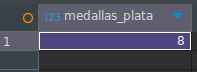
\includegraphics[width=10cm]{resources/resultados/r7.png}
\end{center}   

Nota: Para obtener este resultado, se añadieron manualmente registros en la tabla Medalla para asegurar que Japón tenga medallas de plata registradas. \vspace{.3cm}
        \item \textbf{El número de medallas de bronce ganadas por España.}\vspace{.3cm}

Ahora similar al caso anterior realizamos lo analogo pero para España: \vspace{.3cm}

\begin{lstlisting}
    SELECT 
    COUNT(*) AS medallas_bronce
FROM 
    Medalla m
JOIN 
    Atleta a ON m.IDAtleta = a.IDAtleta
WHERE 
    a.NombrePais = 'Espana' AND m.TipoMedalla = 'Bronce';
\end{lstlisting}

\vspace{.3cm}

En esta consulta, seleccionamos la tabla Medalla para contar el número de medallas de bronce ganadas por España. Utilizamos la función COUNT(*) para contar todas las filas que cumplen con las condiciones especificadas en el WHERE, es decir, aquellas donde el país es 'España' y el tipo de medalla es 'Bronce'. \vspace{.3cm}

El resultado es un solo valor que representa el número total de medallas de bronce ganadas por España \textit{(analogo al inciso anterior)}. \vspace{.3cm}

\textbf{Resultado:}
\begin{center}
    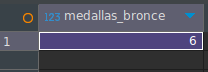
\includegraphics[width=10cm]{resources/resultados/r8.png}
\end{center}   

Nota: Para este resultado, tambien se añadieron manualmente tuplas en la tabla Medalla. \vspace{.3cm}
        \item \textbf{La información de los atletas que ganaron medallas en la disciplina halterofilia.}\vspace{.3cm}

Para esta consulta, lo resolví de la siguiente manera: \vspace{.3cm}

\begin{lstlisting}
    SELECT 
    a.IDAtleta,
    a.Nombre,
    a.PrimerApellido,
    a.SegundoApellido,
    a.FechaNacimiento,
    a.Nacionalidad,
    a.Genero,
    m.TipoMedalla
FROM 
    Medalla m
JOIN 
    Atleta a ON m.IDAtleta = a.IDAtleta
JOIN 
    Disciplina d ON m.IDDisciplina = d.IDDisciplina
WHERE 
    d.NombreDisciplina = 'Halterofilia';
\end{lstlisting}

\textbf{Explicación:} \vspace{.3cm}

En esta consulta, seleccionamos la tabla `atleta` para obtener la información de los atletas que han ganado medallas en la disciplina de halterofilia. Utilizamos un `JOIN` con la tabla `medalla` para relacionar los atletas con las medallas que han ganado. Luego, filtramos los resultados para incluir solo aquellos donde la disciplina de la medalla es 'Halterofilia'. \vspace{.3cm}

El resultado es un conjunto de filas que representan a los atletas que han ganado medallas en la disciplina de halterofilia. \vspace{.3cm}

\textbf{Resultado:}
\begin{center}
    
\end{center}   

Nota: Para este resultado, se añadieron manualmente tuplas en la tabla `medalla` para asegurar que haya registros de medallas en la disciplina de halterofilia. \vspace{.3cm}
        \item \begin{center}
	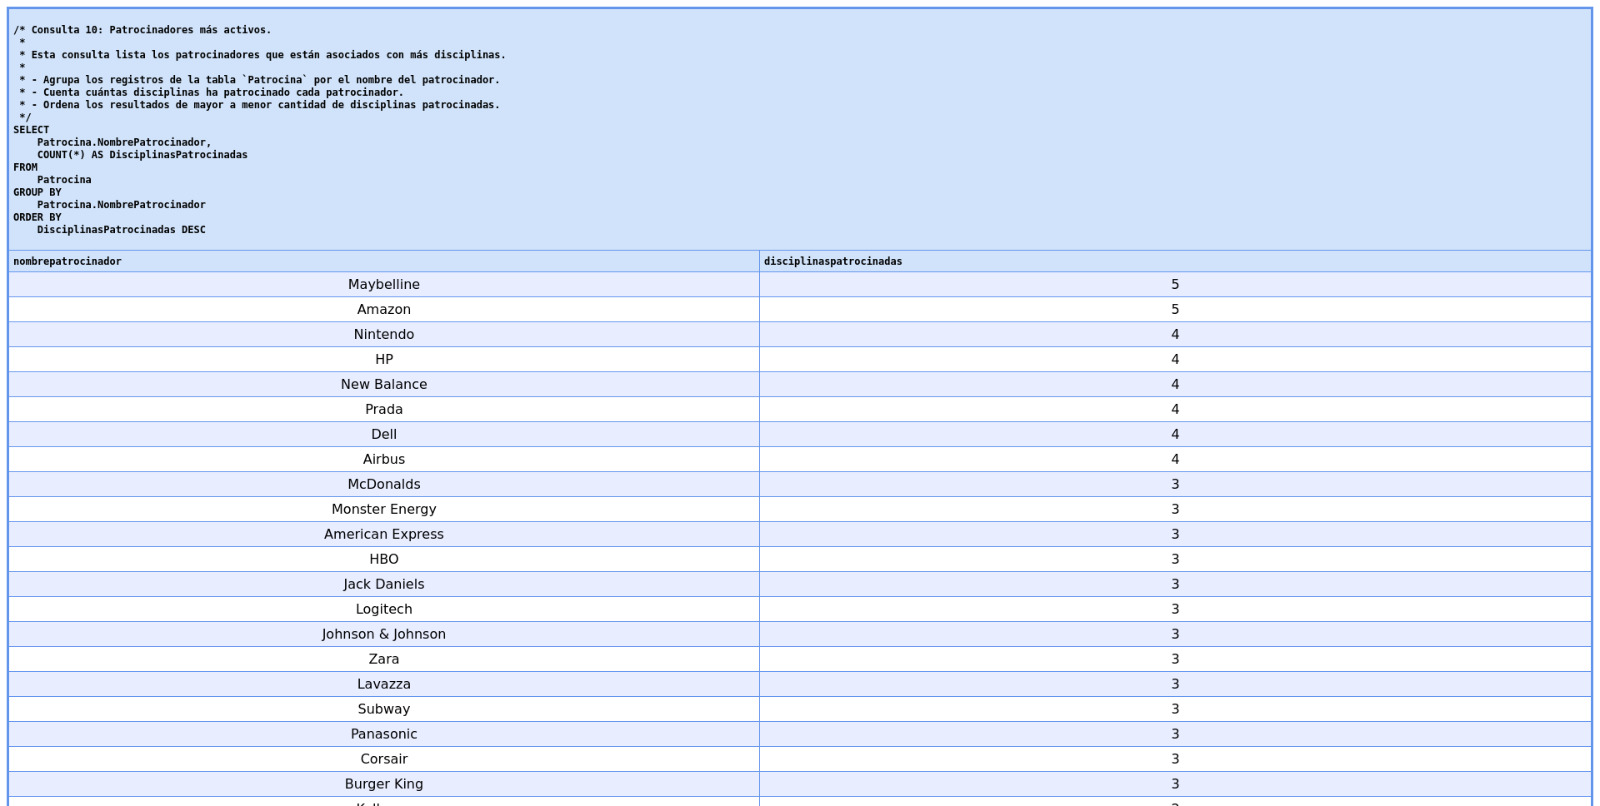
\includegraphics[width=16.5cm]{resources/Chapters/Consultas/Imagenes/Consulta10.jpg} 
	
	Consulta 10. Patrocinadores más activos. 
\end{center}

\textbf{Propósito de la consulta}

La consulta tiene como objetivo identificar a los patrocinadores más activos, es decir, aquellos que están asociados con la mayor cantidad de disciplinas patrocinadas. Los resultados se ordenan de mayor a menor según el número de disciplinas patrocinadas.

\textbf{Desglose de la consulta}

\begin{itemize} \item \textbf{Selección de columnas (\texttt{SELECT}):} \begin{itemize} \item \texttt{Patrocina.NombrePatrocinador}: Nombre del patrocinador, que identifica de forma única a cada entidad patrocinadora. \item \texttt{COUNT(*) AS DisciplinasPatrocinadas}: Cuenta el número total de disciplinas patrocinadas por cada patrocinador. \end{itemize}
	
	\item \textbf{Tabla involucrada (\texttt{FROM}):} \begin{itemize} \item \texttt{Patrocina}: Tabla que almacena la relación entre patrocinadores y disciplinas patrocinadas. \end{itemize}
	
	\item \textbf{Agrupación de resultados (\texttt{GROUP BY}):} \begin{itemize} \item \texttt{Patrocina.NombrePatrocinador}: Agrupa los registros por el nombre del patrocinador para calcular cuántas disciplinas ha patrocinado cada uno. \end{itemize}
	
	\item \textbf{Ordenamiento de resultados (\texttt{ORDER BY}):} \begin{itemize} \item Los resultados se ordenan por \texttt{DisciplinasPatrocinadas} en orden descendente (\texttt{DESC}), de modo que los patrocinadores más activos aparezcan primero. \end{itemize} \end{itemize}

\textbf{Análisis detallado}

\begin{itemize} \item \textbf{Relación entre patrocinadores y disciplinas:} \begin{itemize} \item La tabla \texttt{Patrocina} registra las asociaciones entre los patrocinadores y las disciplinas que apoyan, lo que permite calcular la cantidad de disciplinas patrocinadas por cada patrocinador. \end{itemize}
	
	\item \textbf{Uso de la función agregada \texttt{COUNT}:} \begin{itemize} \item \texttt{COUNT(*)} cuenta el número total de registros asociados con cada patrocinador, lo que representa el número de disciplinas que han patrocinado. \end{itemize}
	
	\item \textbf{Agrupación por patrocinador:} \begin{itemize} \item La agrupación por \texttt{Patrocina.NombrePatrocinador} asegura que el conteo de disciplinas patrocinadas sea específico para cada patrocinador. \end{itemize}
	
	\item \textbf{Ordenamiento por actividad:} \begin{itemize} \item Ordenar los resultados por \texttt{DisciplinasPatrocinadas} permite identificar fácilmente a los patrocinadores más activos. \end{itemize} \end{itemize}

\textbf{Posibles escenarios y consideraciones}

\begin{itemize} \item \textbf{Patrocinadores sin disciplinas asociadas:} \begin{itemize} \item Si un patrocinador no tiene disciplinas asociadas en la tabla \texttt{Patrocina}, no aparecerá en los resultados, ya que \texttt{COUNT(*)} excluye registros inexistentes. \end{itemize}
	
	\item \textbf{Empates en la actividad:} \begin{itemize} \item Si dos o más patrocinadores tienen la misma cantidad de disciplinas patrocinadas, el orden relativo entre ellos no está definido. \end{itemize}
	
	\item \textbf{Interpretación de los resultados:} \begin{itemize} \item La consulta solo refleja la cantidad de disciplinas patrocinadas, pero no considera otros factores como la inversión o la duración del patrocinio. \end{itemize} \end{itemize}

La consulta proporciona una lista clara de los patrocinadores más activos en términos de disciplinas apoyadas, lo que puede ser útil para evaluar la participación y el impacto de los patrocinadores en el evento.
    \end{enumerate}
    \end{section}


% bibliografia    
% \printbibliography
  
\end{document}